\section{Win32 PE}
\label{win32_pe}
\myindex{Windows!Win32}

\acs{PE} is an executable file format used in Windows.
The difference between .exe, .dll and .sys is that .exe and .sys usually do not have exports, only imports.

\myindex{OEP}

A \ac{DLL}, just like any other PE-file, has an entry point (\ac{OEP}) (the function DllMain() is located there) 
but this function usually does nothing.
.sys is usually a device driver.
As of drivers, Windows requires the checksum to be present in the PE file and for it to be correct
\footnote{For example, Hiew(\myref{Hiew}) can calculate it}.

\myindex{Windows!Windows Vista}
Starting at Windows Vista, a driver's files must also be signed with a digital signature. It will fail to load otherwise.

\myindex{MS-DOS}
Every PE file begins with tiny DOS program that prints a
message like \q{This program cannot be run in DOS mode.}---if you run this program in DOS or Windows 3.1 (\ac{OS}-es which are not aware of the PE format), 
this message will be printed.

\subsection{Terminology}

\myindex{VA}
\myindex{Base address}
\myindex{RVA}
\myindex{Windows!IAT}
\myindex{Windows!INT}

\begin{itemize}
\item Module---a separate file, .exe or .dll.

\item Process---a program loaded into memory and currently running.  Commonly consists of one .exe file and bunch of .dll files.

\item Process memory---the memory a process works with.  Each process has its own.
There usually are loaded modules, memory of the stack, \gls{heap}(s), etc.

\item \ac{VA}---an address which is to be used in program while runtime.

\item Base address (of module)---the address within the process memory at which the module is to be loaded.
\ac{OS} loader may change it, if the base address is already occupied by another module just loaded before.

\item \ac{RVA}---the \ac{VA}-address minus the base address.

Many addresses in PE-file tables use \ac{RVA}-addresses.

%\item
%Data directory\EMDASH{}...

\item \ac{IAT}---an array of addresses of imported symbols \footnote{\PietrekPE}. 
Sometimes, the \TT{IMAGE\_DIRECTORY\_ENTRY\_IAT} data directory points at the \ac{IAT}. 
\label{IDA_idata}
It is worth noting that \ac{IDA} (as of 6.1) may allocate a pseudo-section named \TT{.idata} for
\ac{IAT}, even if the \ac{IAT} is a part of another section!

\item \ac{INT}---an array of names of symbols to be imported\footnote{\PietrekPE}.
\end{itemize}

\subsection{Base address}

The problem is that several module authors can prepare DLL files for others to use and it is not possible
to reach an agreement which addresses is to be assigned to whose modules.

So that is why if two necessary DLLs for a process have the same base address,
one of them will be loaded at this base address, and the other---at some other free space in process memory,
and each virtual addresses in the second DLL will be corrected.

\par Often, \ac{MSVC} the linker generates the .exe files with a base address of \TT{0x400000}
\footnote{The origin of this address choice is described here: \href{http://go.yurichev.com/17041}{MSDN}},
and with the code section starting at \TT{0x401000}.
This mean that the \ac{RVA} of the start of the code section is \TT{0x1000}.

DLLs are often generated by MSVC's linker with a base address of \TT{0x10000000}
\footnote{This can be changed by the /BASE linker option}.

\myindex{ASLR}

There is also another reason to load modules at various base addresses, in this case random ones.
It is \ac{ASLR}\footnote{\href{http://go.yurichev.com/17140}{wikipedia}}.

\myindex{Shellcode}

A shellcode trying to get executed on a compromised system must call system functions, hence, know their addresses.

In older \ac{OS} (in \gls{Windows NT} line: before Windows Vista),
system DLL (like kernel32.dll, user32.dll) were always loaded at known addresses, 
and if we also recall
that their versions rarely changed, the addresses of functions were
fixed and shellcode could call them directly.

In order to avoid this, the \ac{ASLR}
method loads your program and all modules it needs at random base addresses, different every time.

\ac{ASLR} support is denoted in a PE file by setting the flag
\par \TT{IMAGE\_DLL\_CHARACTERISTICS\_DYNAMIC\_BASE} (see: [\Russinovich]).

\subsection{Subsystem}

There is also a \IT{subsystem} field, usually it is:

\myindex{Native API}

\begin{itemize}
\item native\footnote{Meaning, the module use Native API instead of Win32} (.sys-driver), 

\item console (console application) or

\item \ac{GUI} (non-console).
\end{itemize}

\subsection{OS version}

A PE file also specifies the minimal Windows version it needs in order to be loadable.

The table of version numbers stored in the PE file and corresponding Windows codenames is
here\footnote{\href{http://go.yurichev.com/17044}{wikipedia}}.

\myindex{Windows!Windows NT4}
\myindex{Windows!Windows 2000}
For example, \ac{MSVC} 2005 compiles .exe files for running on Windows NT4 (version 4.00), but \ac{MSVC} 2008 does not 
(the generated files have a version of 5.00, at least Windows 2000 is needed to run them).

\myindex{Windows!Windows XP}

\ac{MSVC} 2012 generates .exe files of version 6.00 by default, 
targeting at least Windows Vista. 
However, by changing the compiler's options\footnote{\href{http://go.yurichev.com/17045}{MSDN}},
it is possible to force it to compile for Windows XP.

\subsection{Sections}

Division in sections, as it seems, is present in all executable file formats.

It is devised in order to separate code from data, and data---from constant data.

\begin{itemize}
\item Either the \IT{IMAGE\_SCN\_CNT\_CODE} or \IT{IMAGE\_SCN\_MEM\_EXECUTE} flags will be set on the code section---this is executable code.

\item On data section\EMDASH\IT{IMAGE\_SCN\_CNT\_INITIALIZED\_DATA}, 
\IT{IMAGE\_SCN\_MEM\_READ} \AndENRU \IT{IMAGE\_SCN\_MEM\_WRITE} flags.

\item On an empty section with uninitialized 
data\EMDASH\IT{IMAGE\_SCN\_CNT\_UNINITIALIZED\_DATA}, \IT{IMAGE\_SCN\_MEM\_READ} \AndENRU \IT{IMAGE\_SCN\_MEM\_WRITE}.

\item On a constant data section (one that's protected from writing), the flags \\
\IT{IMAGE\_SCN\_CNT\_INITIALIZED\_DATA} and \IT{IMAGE\_SCN\_MEM\_READ} can be set, but not \IT{IMAGE\_SCN\_MEM\_WRITE}. 
A process going to crash if it tries to write to this section.
\end{itemize}

\myindex{TLS}
\myindex{BSS}
Each section in PE-file may have a name, however, it is not very important.
Often (but not always) the code section is named \TT{.text}, 
the data section\EMDASH{}\TT{.data}, the constant data section --- \TT{.rdata} \IT{(readable data)}.
Other popular section names are: 

\myindex{MIPS}
\begin{itemize}
\item \TT{.idata}---imports section.
\ac{IDA} may create a pseudo-section named like this: \myref{IDA_idata}.
\item \TT{.edata}---exports section (rare)
\item \TT{.pdata}-section containing all information about exceptions in Windows NT for MIPS, \ac{IA64} and x64: \myref{SEH_win64}
\item \TT{.reloc}---relocs section
\item \TT{.bss}---uninitialized data (\ac{BSS})
\item \TT{.tls}---thread local storage (\ac{TLS})
\item \TT{.rsrc}---resources
\item \TT{.CRT}---may present in binary files compiled by ancient MSVC versions
\end{itemize}

PE file packers/encryptors often garble section names or replace the names with their own.

\ac{MSVC} allows you to declare data in arbitrarily named section
\footnote{\href{http://go.yurichev.com/17047}{MSDN}}.

Some compilers and linkers can add a section with debugging symbols and 
other debugging information (MinGW for instance).
\myindex{Windows!PDB}
However it is not so in modern versions of \ac{MSVC} (separate \gls{PDB} files are used there for this purpose).\\
\\
That is how a PE section is described in the file:

\begin{lstlisting}
typedef struct _IMAGE_SECTION_HEADER {
  BYTE  Name[IMAGE_SIZEOF_SHORT_NAME];
  union {
    DWORD PhysicalAddress;
    DWORD VirtualSize;
  } Misc;
  DWORD VirtualAddress;
  DWORD SizeOfRawData;
  DWORD PointerToRawData;
  DWORD PointerToRelocations;
  DWORD PointerToLinenumbers;
  WORD  NumberOfRelocations;
  WORD  NumberOfLinenumbers;
  DWORD Characteristics;
} IMAGE_SECTION_HEADER, *PIMAGE_SECTION_HEADER;
\end{lstlisting}
\footnote{\href{http://go.yurichev.com/17048}{MSDN}}

\myindex{Hiew}
A word about terminology: \IT{PointerToRawData} it called \q{Offset} in Hiew
and \IT{VirtualAddress} is called \q{RVA} there.

\subsection{Relocations (relocs)}
\label{subsec:relocs}

\ac{AKA} FIXUP-s (at least in Hiew).

They are also present in almost all executable file formats
\footnote{Even in .exe files for MS-DOS}.
Exceptions are shared dynamic libraries compiled with \ac{PIC}, or any other \ac{PIC}-code.

What are they for?

Obviously, modules can be loaded on various base addresses, but how to deal with global variables, for example?
They must be accessed by address.  One solution is \PICcode{} (\myref{sec:PIC}).
But it is not always convenient.

That is why a relocations table is present.
There the addresses of points that need to be corrected are enumerated, 
in case of loading at a different base address.

% TODO тут бы пример с HIEW или objdump..
For example, there is a global variable at address \TT{0x410000} and this is how it is accessed:

\begin{lstlisting}
A1 00 00 41 00         mov         eax,[000410000]
\end{lstlisting}

The base address of the module is \TT{0x400000}, the \ac{RVA} of the global variable is \TT{0x10000}.

If the module is loaded at base address \TT{0x500000}, the real address of the global variable must be \TT{0x510000}.

\myindex{x86!\Instructions!MOV}

As we can see, the address of variable is encoded in the instruction \TT{MOV}, after the byte \TT{0xA1}.

That is why the address of the 4 bytes after \TT{0xA1}, is written in the relocs table.

If the module is loaded at a different base address, the \ac{OS} loader enumerates all addresses in the table, 

finds each 32-bit word the address points to, subtracts the original base address from it
(we get the \ac{RVA} here), and adds the new base address to it.

If a module is loaded at its original base address, nothing happens.

All global variables can be treated like that.

Relocs may have various types, however, in Windows for x86 processors, the type is usually \\
\IT{IMAGE\_REL\_BASED\_HIGHLOW}.

\myindex{Hiew}

By the way, relocs are darkened in Hiew, for example: \figref{fig:scanf_ex3_hiew_1}.

\myindex{\olly}
\olly underlines the places in memory to which relocs are to be applied, for example: \figref{fig:switch_lot_olly3}.

\subsection{Exports and imports}

\label{PE_exports_imports}
As we all know, any executable program must use the \ac{OS}'s services and other DLL-libraries somehow.

It can be said that functions from one module (usually DLL) must be connected somehow to the points of their
calls in other modules (.exe-file or another DLL).

For this, each DLL has an \q{exports} table, which consists of functions plus their addresses in a module.

And every .exe file or DLL has \q{imports}, a table of functions it needs for execution including
list of DLL filenames.

After loading the main .exe-file, the \ac{OS} loader processes imports table: 
it loads the additional DLL-files, finds function names
among the DLL exports and writes their addresses down in the \ac{IAT} of the main .exe-module.

\myindex{Windows!Win32!Ordinal}

As we can see, during loading the loader must compare a lot of function names, but string comparison is not a very
fast procedure, so there is a support for \q{ordinals} or \q{hints},
which are function numbers stored in the table, instead of their names.

That is how they can be located faster when loading a DLL.
Ordinals are always present in the \q{export} table.

\myindex{MFC}
For example, a program using the \ac{MFC} library usually loads mfc*.dll by ordinals,
and in such programs there are no \ac{MFC} function names in \ac{INT}.

% TODO example!
When loading such programs in \IDA, it will ask for a path to the mfc*.dll files
in order to determine the function names.

If you don't tell \IDA the path to these DLLs, there will be \IT{mfc80\_123} instead of function names.

\subsubsection{Imports section}

Often a separate section is allocated for the imports table and everything related to it (with name like \TT{.idata}),
however, this is not a strict rule.

Imports are also a confusing subject because of the terminological mess. Let's try to collect all information in one place.

\begin{figure}[H]
\centering
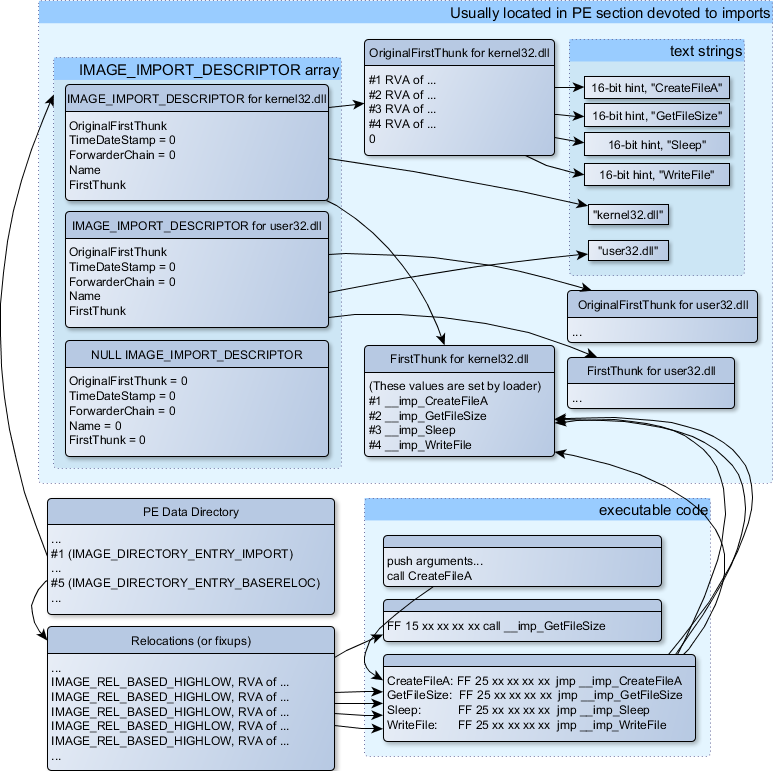
\includegraphics[scale=\FigScale]{OS/PE/unnamed0.png}
\caption{
A scheme that unites all PE-file structures related to imports}
\end{figure}

The main structure is the array \IT{IMAGE\_IMPORT\_DESCRIPTOR}.
Each element for each DLL being imported.

Each element holds the \ac{RVA} address of the text string (DLL name) (\IT{Name}).

\IT{OriginalFirstThink} is the \ac{RVA} address of the \ac{INT} table. 
This is an array of \ac{RVA} addresses, each of which points to a text string with a function name. 
Each string is prefixed by a 16-bit integer 
(\q{hint})---\q{ordinal} of function.

While loading, if it is possible to find a function by ordinal,
then the strings comparison will not occur. The array is terminated by zero.

There is also a pointer to the \ac{IAT} table named \IT{FirstThunk}, it is just the \ac{RVA} address 
of the place where the loader writes the addresses of the resolved functions.

The points where the loader writes addresses are marked by \IDA like this: \IT{\_\_imp\_CreateFileA}, etc.

There are at least two ways to use the addresses written by the loader.

\myindex{x86!\Instructions!CALL}
\begin{itemize}
\item The code will have instructions like \IT{call \_\_imp\_CreateFileA}, 
and since the field with the address of the imported function is a global variable in some sense, 
the address of the \IT{call} instruction (plus 1 or 2) is to be added to the relocs table,
for the case when the module is loaded at a different base address.

But, obviously, this may enlarge relocs table significantly.

Because there are might be a lot of calls to imported functions in the module.

Furthermore, large relocs table slows down the process of loading modules.

\myindex{x86!\Instructions!JMP}
\myindex{thunk-functions}
\item For each imported function, there is only one jump allocated, using the \JMP instruction 
plus a reloc to it.
Such points are also called \q{thunks}.

All calls to the imported functions are just \CALL instructions to the corresponding \q{thunk}.
In this case, additional relocs are not necessary because these CALL-s
have relative addresses and do not need to be corrected.
\end{itemize}

These two methods can be combined.

Possible, the linker creates individual \q{thunk}s if there are too many calls to the function,
but not done by default. \\
\\
By the way, the array of function addresses to which FirstThunk is pointing is not necessary to be located in the \ac{IAT} section.
For example, author of these lines once wrote the PE\_add\_import\footnote{\href{http://go.yurichev.com/17049}{yurichev.com}} 
utility for adding imports to an existing .exe-file.

Some time earlier, in the previous versions of the utility, 
at the place of the function you want to substitute with a call to another DLL,
my utility wrote the following code:

\begin{lstlisting}
MOV EAX, [yourdll.dll!function]
JMP EAX
\end{lstlisting}

FirstThunk points to the first instruction. In other words, when loading yourdll.dll,
the loader writes the address of the \IT{function} function right in the code.

It also worth noting that a code section is usually write-protected, so my utility adds the \\
\IT{IMAGE\_SCN\_MEM\_WRITE} 
flag for code section. Otherwise, the program to crash while loading with error code
5 (access denied). \\
\\
One might ask: what if I supply a program with a set of DLL files which is not supposed to change (including addresses of all DLL functions),
is it possible to speed up the loading process?

Yes, it is possible to write the addresses of the functions to be imported into the FirstThunk arrays in advance.
The \IT{Timestamp} field is present in the \\
\IT{IMAGE\_IMPORT\_DESCRIPTOR} structure.

If a value is present there, then the loader compares this value with the date-time of the DLL file.

If the values are equal, then the loader does not do anything, and the loading of the process can be faster.
This is called \q{old-style binding}
\footnote{\href{http://go.yurichev.com/17050}{MSDN}. There is also the \q{new-style binding}.}.
\myindex{BIND.EXE}

The BIND.EXE utility in Windows SDK is for for this.
For speeding up the loading of your program, Matt Pietrek in \PietrekPEURL, suggests to do the binding shortly after your program
installation on the computer of the end user. \\
\\
PE-files packers/encryptors may also compress/encrypt imports table.

In this case, the Windows loader, of course, will not load all necessary DLLs.
\myindex{Windows!Win32!LoadLibrary}
\myindex{Windows!Win32!GetProcAddress}

Therefore, the packer/encryptor does this on its own, with the help of 
\IT{LoadLibrary()} and the \IT{GetProcAddress()} functions.

That is why these two functions are often present in \ac{IAT} in packed files.\\
\\
In the standard DLLs from the Windows installation, \ac{IAT} often is located right in the beginning of the PE file.
Supposedly, it is done for optimization.

While loading, the .exe file is not loaded into memory as a whole (recall huge install programs which are
started suspiciously fast), it is \q{mapped}, and loaded into memory in parts as they are accessed.

Probably, Microsoft developers decided it will be faster.

\subsection{Resources}

\label{PEresources}

Resources in a PE file are just a set of icons, pictures, text strings, dialog descriptions.

Perhaps they were separated from the main code, so all these things could be multilingual,
and it would be simpler to pick text or picture for the language that is currently set in the \ac{OS}. \\
\\
As a side effect, they can be edited easily and saved back to the executable file, even if one does not have special knowledge, 
by using the ResHack editor, for example (\myref{ResHack}).

\subsection{.NET}

\myindex{.NET}

.NET programs are not compiled into machine code but into a special bytecode.
\myindex{OEP}
Strictly speaking, there is bytecode instead of the usual x86 code
in the .exe file, however, the entry point (\ac{OEP}) points to this tiny fragment of x86 code:

\begin{lstlisting}
jmp         mscoree.dll!_CorExeMain
\end{lstlisting}

The .NET loader is located in mscoree.dll, which processes the PE file.
\myindex{Windows!Windows XP}

It was so in all pre-Windows XP \ac{OS}es. Starting from XP, the \ac{OS} loader is able to detect the .NET file
and run it without executing that \JMP instruction
\footnote{\href{http://go.yurichev.com/17051}{MSDN}}.

\myindex{TLS}
\subsection{TLS}

This section holds initialized data for the \ac{TLS}(\myref{TLS}) (if needed).
When a new thread start, its \ac{TLS} data is initialized using the data from this section. \\
\\
\myindex{TLS!Callbacks}

Aside from that, the PE file specification also provides initialization of the
\ac{TLS} section, the so-called TLS callbacks.

If they are present, they are to be called before the control is passed to the main entry point (\ac{OEP}).

This is used widely in the PE file packers/encryptors.

\subsection{Tools}

\myindex{objdump}
\myindex{Cygwin}
\myindex{Hiew}
\label{ResHack}

\begin{itemize}
\item objdump (present in cygwin) for dumping all PE-file structures.

\item Hiew(\myref{Hiew}) as editor.

\item pefile---Python-library for PE-file processing \footnote{\url{http://go.yurichev.com/17052}}.

\item ResHack \acs{AKA} Resource Hacker---resources editor\footnote{\url{http://go.yurichev.com/17052}}.

\item PE\_add\_import\footnote{\url{http://go.yurichev.com/17049}}---
simple tool for adding symbol(s) to PE executable import table.

\item PE\_patcher\footnote{\href{http://go.yurichev.com/17054}{yurichev.com}}---simple tool for patching PE executables.

\item PE\_search\_str\_refs\footnote{\href{http://go.yurichev.com/17055}{yurichev.com}}---simple tool for searching for a function in PE executables which use some text string.
\end{itemize}

\subsection{Further reading}

% FIXME: bibliography per chapter or section
\begin{itemize}
\item Daniel Pistelli---The .NET File Format \footnote{\url{http://go.yurichev.com/17056}}
\end{itemize}

